% Load the kaohandt class (with the default options)
\documentclass[
	fontsize=10pt, % Base font size
	%twoside=false, % If true, use different layouts for even and odd pages (in particular, if twoside=true, the margin column will be always on the outside)
	%secnumdepth=2, % How deep to number headings. Defaults to 2 (subsections)
	abstract=true, % Uncomment to print the title of the abstract
]{kaohandt}

% Choose the language
\usepackage[english]{babel} % Load characters and hyphenation
\usepackage[english=british]{csquotes}	% English quotes


\graphicspath{{Figures/}} % Paths where images are looked for

% Load mathematical packages for theorems and related environments.
\usepackage{kaotheorems}

% Load the package for hyperreferences
\usepackage{kaorefs}

\usepackage{graphicx}
\usepackage{tikzpagenodes} % gives current page anchors

% logo on every page (top-right margin)
\AddToHook{shipout/foreground}{%
  \begin{tikzpicture}[remember picture,overlay]
    \node[anchor=north, inner sep=40pt]
      at (current page.north)
        {
\includegraphics[width=1.5\textwidth]{Logo_USM_SEEE}}; % from \graphicspath
  \end{tikzpicture}%
}
\newcommand{\coursebadge}{%
  \begin{tikzpicture}[remember picture,overlay]
    % yshift controls vertical position from the top edge
    \node[anchor=north] at ([yshift=-40mm,xshift=50mm]current page.north) {%
      \begin{minipage}{50mm}\raggedleft\rmfamily
        {\Huge \bfseries EEM441}\\[0.40em]
        {\Large SEMESTER I}\\[0.40em]
        {\Large(2025/2026)}
      \end{minipage}
    };
  \end{tikzpicture}%
}
\usepackage{marginnote}
\usepackage[most]{tcolorbox}

% margin card style
\newtcolorbox{_margincard}[1][]{
  enhanced,
  colback=blue!6,      % fill color
  colframe=blue!60!black,
  boxrule=0.6pt,
  arc=2mm,
  left=7pt,right=7pt,top=6pt,bottom=6pt,
  width=\dimexpr\marginparwidth-2pt\relax,
  #1
}
% Style for the colored margin box
\newtcolorbox{marginCard}[1][]{
  enhanced, colback=blue!6, colframe=blue!60!black,
  boxrule=0.6pt, arc=2mm,
  left=6pt,right=6pt,top=6pt,bottom=6pt,
  width=\marginparwidth, % match margin width
  #1
}

% Place a margin box under the side ToC (right margin, first page by default)
% #1 = vertical offset from the top edge (default 65mm)
\newcommand{\marginboxbelowtoc}[2][65mm]{%
  \begin{tikzpicture}[remember picture,overlay]
    % anchor at outer top corner; move left by marginparsep and down by #1
    \node[anchor=north east, xshift=-22mm, yshift=-125mm]
      at (current page.north east)
      {\begin{marginCard}#2\end{marginCard}};
  \end{tikzpicture}%
}
% If the box appears in the inner margin, toggle:
% \reversemarginpar   % outer margin in twoside docs

\usepackage{enumitem}
\usepackage{caption}

\DeclareCaptionFormat{ontop}{#1#2#3}
%----------------------------------------------------------------------------------------

\begin{document}

%----------------------------------------------------------------------------------------
%	REPORT INFORMATION
%----------------------------------------------------------------------------------------

\title{Experiment 1 \\ DC Motor / PID Control}

\author[FA]{Farhan Aizuddin}

\date{\today}

%----------------------------------------------------------------------------------------
%	TITLE AND ABSTRACT
%----------------------------------------------------------------------------------------

\maketitle
\coursebadge
\margintoc

\begin{abstract}
\noindent
This experiment covers the basics of DC motor and PID control. The objectives of this experiment are to understand the working principle of a DC motor, to learn how to control the speed and position of a DC motor using PID control, and to implement a PID controller. The experiment involves setting up a DC motor system, tuning the PID controller parameters, and analyzing the performance of the control system.
\end{abstract}

{\noindent\textbf{Keywords:} DC motor, PID control}

\medskip

%----------------------------------------------------------------------------------------
%	MAIN BODY
%----------------------------------------------------------------------------------------

\section{Introduction}
This experiment focuses on the study of DC motors and the implementation of PID control to regulate their speed and position. A DC motor is an electromechanical device that converts electrical energy into mechanical energy through the interaction of magnetic fields. PID control is a widely used control strategy that combines proportional, integral, and derivative actions to achieve desired system performance. The experiment aims to provide hands-on experience in setting up a DC motor system, tuning PID controller parameters, and analyzing the system's response to various inputs.

\marginboxbelowtoc[70mm]{%
\textbf{Objectives:}\par
\begin{enumerate}[label=\alph*), leftmargin=1.2em, labelsep=.4em,
                  itemsep=.20em, topsep=.15em, parsep=0pt]
    \item To study the Open-Loop Speed Control of a DC Motor.
    \item To study the Closed-Loop Speed Control using:
    \begin{enumerate}[label=\Alph*), widest=D, leftmargin=*, labelsep=.4em,
                  itemsep=.15em, topsep=.08em, parsep=0pt]
      \item P Controller
      \item PD Controller
      \item PI Controller
      \item PID Controller
    \end{enumerate}
\end{enumerate}
\textbf{Apparatus Required:}
\begin{enumerate}[label=\arabic*., leftmargin=1.2em, labelsep=.4em,
                  itemsep=.18em, topsep=.12em, parsep=0pt]
    \item Controller kit
    \item Cathode ray \\ oscilloscope
    \item BNC connectors with cords
    \item Multimeter
\end{enumerate}
}

\section{Methodology}
\subsection{Open-Loop Speed Control of a DC Motor}
\begin{enumerate}
    \item Switch on supply and measure all constant voltages and calibrate variable voltages in terms of voltages and angles in degrees.
    \item Disconnect all cable wires from the hardware module.
    \item Make circuitry as shown in Figure \ref{openloop} for the implementation of open-loop speed control of a DC motor.
    \item Connect \textbf{\emph{Output A}} of the motor plant to channel 2 of the oscilloscope.
\end{enumerate}
        {%
        \floatsetup[figure]{ % float  for figures
            capposition=below,% <<<<<
            margins=centering,%
            floatwidth=\textwidth%
        }
        \captionsetup[figure]{% Local captions style
            format=ontop,% use this style
            singlelinecheck=false,%
            justification=centering,
            aboveskip=3pt,%
            belowskip=3pt,%
            font=footnotesize%
        }
        \begin{figure}[H]
            \centering
            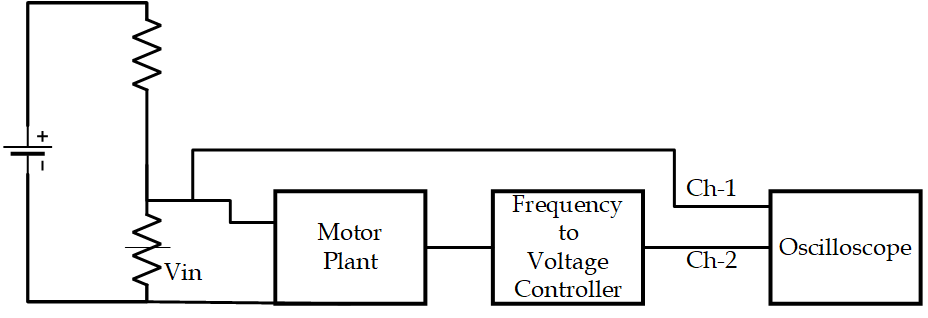
\includegraphics[width=\textwidth]{OpenLoopMotorControl.png}
            %\caption{This caption is centered and placed on top the figure.}
            \label{openloop}
        \end{figure}
\appendix % From here onwards, chapters are numbered with letters, as is the appendix convention

\section{Appendix}



\end{document}
